\newpage
\section{Émulation de périphériques}
\subsection{Environnement Qemu et machine Reptar}
Cette étape vous permet de vous familiariser avec l’environnement que nous utiliserons pour
l’émulation de périphériques.
Dans cette étape, il est nécessaire de travailler avec l'application graphique Qtemu, qui constitue le
frontend graphique de Qemu. L'application est développée en C++ et utilise la librairie Qt. \\\\
\textbf{a) Donnée: }A partir du répertoire seee\_student, lancez le frontend graphique avec le script stq \\\\
\textbf{Travail réalisé: }
\begin{lstlisting}
$ cd ~/seee_student/
$ ./stq
...
Reptar # 
\end{lstlisting}
\begin{figure}[H]
	\begin{center}
		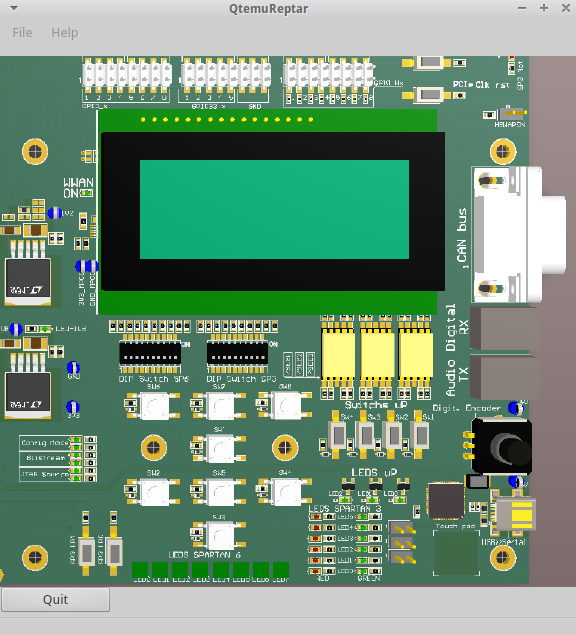
\includegraphics[width=10cm]{img/emulation1.png}
		\caption{Frontend graphique de Qemu}
		\label{emulation1}
	\end{center}
\end{figure}
\textbf{b) Donnée: }Les fichiers sources de Qemu se trouvent dans le répertoire qemu-reds. Examinez les fichiers
suivants :
\begin{enumerate}
	\item hw/arm/reptar/reptar.c Emulation plate-forme REPTAR
	\item hw/reptar\_sp6.c Emulation de la FPGA
	\item hw/reptar\_sp6\_clcd.c Emulation gestion du LCD4x20
	\item hw/reptar\_sp6\_buttons.c Emulation gestion des boutons
	\item hw/reptar\_sp6\_emul.c Gateway entre Qemu et Qtemu
\end{enumerate}
Vous trouverez également toute la documentation nécessaire sur la plate-forme Reptar dans le
répertoire doc. \\\\
\textbf{Remarque: }Ces différents fichiers implémentent ce qui ressemble à des modules noyaux.\\\\
\textbf{c) Donnée: } La compilation de Qemu pourra s'effectuer dans le répertoire qemu-reds directement, avec la
commande make (utilisez make -j4 ou -j8 pour aller plus vite !). \\\\
\textbf{Travail réalisé: }Par la suite, seule la commande \textit{make} sera nécessaire pour recompiler l'émulateur.\\
En lançant \textit{./qtemu} et Eclipse, on pourra debugger l'émulateur Qemu.
\begin{lstlisting}
$ cd ~/seee_student/qemu-reds/
$ ./configure --target-list=arm-softmmu --enable-debug --disable-attr --disable-docs 
...
$ make -j8
...
$
\end{lstlisting}
\subsection{Émulation de la FPGA Spartan6}
Dans cette étape, il s'agit de mettre en place la structure nécessaire à l'émulation de la FPGA intégrée
à la plate-forme. La FPGA implémente des registres associés aux périphériques externes. Dans cette
étape, il s'agit de s'assurer que l'accès aux adresses I/O en lecture et écriture fonctionne. \\\\
\textbf{a) Donnée: }Complétez l'émulation de la FPGA afin de tester l'écriture et la lecture à l'une ou l'autre adresse
dédiée à la FPGA (affichez simplement un message). \\\\
\textbf{Emplacement du code:}\\\textit{/emulationSpartan6\_part2/reptar\_sp6.c}\\ \textit{/emulationSpartan6\_part2/reptar.c}\\\\
\textbf{Travail réalisé: }Nous avons modifié les fichiers \textit{reptar\_sp6.c} et \textit{reptar.c}\\
Le point crucial de cette partie du labo a été de trouvé l'adresse de base de la FPGA qui est \textbf{0x18000000}. Nous avons en effet besoin de cette adresse pour lier/créer le \textit{reptar\_sp6} dans la partie reptar. 
\begin{lstlisting}
	sysbus_create_simple("reptar_sp6",0x18000000,NULL);
\end{lstlisting}
Pour le reste de l'implémentation, nous nous somme basé sur le diagramme de séquence du support de cours et avons pris le document \textit{versatilepb.c} comme exemple pour le contenu des méthodes callback.\\
Le bon fonctionnement du code a été "testé" premièrement en réussissant la compilation sans erreurs, puis le lancement sans crash. Nous avons également ajouté des messages affichés dans la console dans les différentes méthodes callback pour suivre l'initialisation. L'exécution a été faite de la manière suivante:
\begin{lstlisting}
$ cd ~/seee_student/qemu-reds/
$ make
...
$ cd ..
$ ./stq
...
sp6 init
reptar-sp6-emul: sp6_emul_init
sp6 initfn
...
Reptar # 
\end{lstlisting}
\textbf{b) Donnée: }Testez les accès en lecture-écriture avec U-Boot. \\\\
\textbf{Travail réalisé: } Pour l'instant, les callback de lecture/écriture que nous avons implémentés contiennent uniquement des messages d'indication qui sont affichés dans la console. À l'aide des commandes suivantes, nous avons pu tester leur bon fonctionnement. Les commandes suivantes tentent de lire, puis écrire à l'adresse de base de la FPGA.
\begin{lstlisting}
Reptar # md.l 0x18000000 1
18000000:sp6 read
 00000000    ....
Reptar # mw.l 0x18000000 1
sp6 write
Reptar #
\end{lstlisting}
\subsection{Émulation des devices de type LED (output)}
\textbf{Donnée: }La FPGA est connectée à des LEDs qui sont visibles sur l'interface graphique. Cette étape consiste à
implémenter le code d'émulation précédent afin de gérer l'accès aux LEDs reliées à la FPGA.
Les interactions entre la FPGA et l'interface graphique doivent être gérées proprement. \\\\
\textbf{Emplacement du code:}\textit{/emulationSpartan6\_part3/reptar\_sp6.c}\\\\
\textbf{Travail réalisé: }Pour cette partie, il a fallu rechercher l'offset du registre des LEDs qui est \textit{0x003A}. Il faut donc ajouter cet offset à l'adresse de base de la FPGA.\\ Nous avons défini une variable qui garde la valeur écrite dans le registre des LEDs pour permettre la relecture de la valeur.\\ Pour la lecture et l'écriture, on teste si l'offset correspond et si l'on lit/écrit des données de la bonne taille, soit 16bits. Des messages ont été implémentés pour indiquer si la lecture/écriture est faite correctement.
\\La valeur lue est simplement affichée dans la console. Pour l'écriture, la valeur écrite est transmise à l'aide d'un message JSON conformément aux directives du \textit{Guide d'utilisation de l'infrastructure}.
\\Nous avons testé le bon fonctionnement du code avec le test 10 de itbok\footnote{itbok, signifie Is The Board OK}. Le test montre que l'on arrive à lire et écrire correctement sur les leds.
\begin{figure}[H]
	\begin{center}
		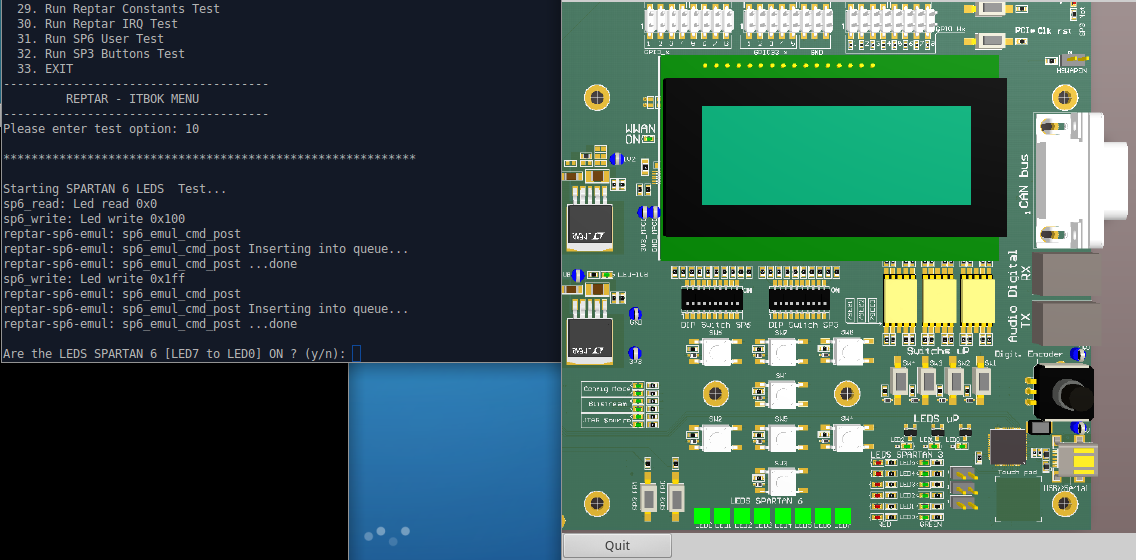
\includegraphics[width=15cm]{img/leds1.png}
		\caption{Test d'allumage des LEDs}
		\label{leds1}
	\end{center}
\end{figure}
\begin{figure}[H]
	\begin{center}
		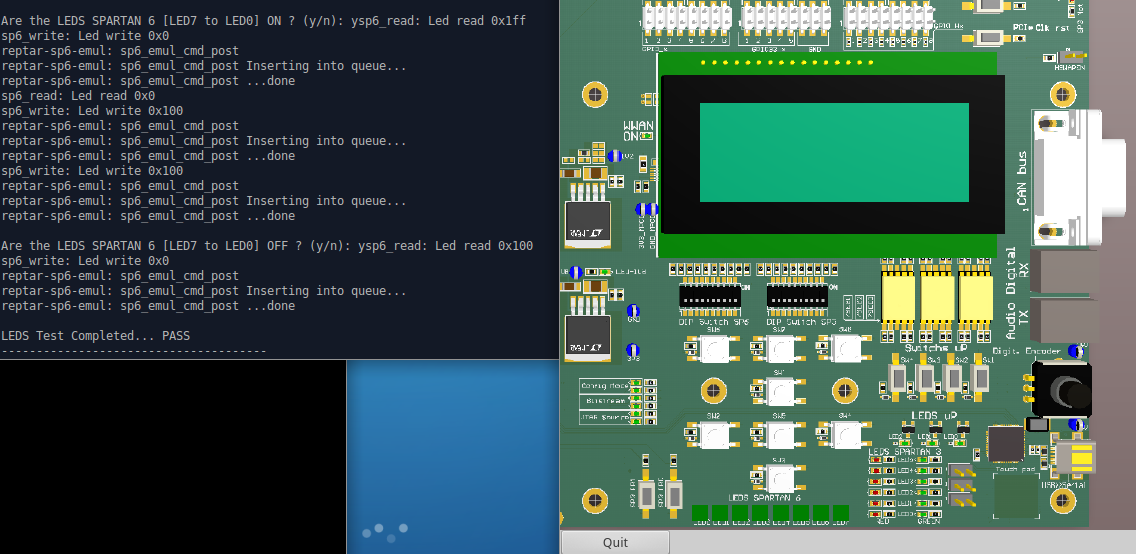
\includegraphics[width=15cm]{img/leds2.png}
		\caption{Test d'extinction des LEDs}
		\label{leds2}
	\end{center}
\end{figure}
\subsection{Émulation de type boutons (input)}
La FPGA est connectée à une série de boutons (switches) sur la plate-forme Reptar. Cette étape consiste
à mettre en place la structure nécessaire à la gestion de ces boutons. \\\\
\textbf{a) Donnée: }Adaptez les fichiers nécessaires afin que l'émulation de votre périphérique (FPGA) puisse détecter
la pression d'une touche, sans vous préoccuper pour le moment des interruptions. \\\\
\textbf{Emplacement du code:}\\\textit{/emulationSpartan6\_part4/reptar\_sp6.c}\\
\textit{/emulationSpartan6\_part4/reptar\_sp6\_buttons.c}\\\\
\textbf{Travail réalisé: }Le code de cette partie est inspiré du \textit{Guide d'utilisation de l'infrastructure}. L'offset pour lire la valeur des boutons est \textit{0x0012}. Lorsqu'un bouton est pressé, le handler du fichier sp6\_button est appelé et la valeur du registre est mémorisée. La valeur des boutons peut également être récupérée lors d'une lecture du registre correspondant.\\\\
\textbf{b) Donnée: }Le projet sp6\_buttons\_u-boot contient une application permettant de tester vos boutons (en mode
polling). Compilez l'application et effectuez quelques tests.\\\\
\textbf{Travail réalisé: }L'application a été compilée avec make. Il faut ensuite lancer l'émulateur avec la commande \textit{stq}. Une fois dans l'U-boot, on peut lancer l'application testant les boutons. Elle est enregistrée dans les variables d'environnements sous le nom \textit{tftp3}. Les lignes ci-dessous démontrent le bon fonctionnement des boutons. Le bouton exit arrête l'application. 
\begin{lstlisting}
$ cd ~/seee_student
$ ./stq
...
Reptar # run tftp3
smc911x: detected LAN9118 controller
smc911x: phy initialized
smc911x: MAC e4:af:a1:40:01:fe
Using smc911x-0 device
TFTP from server 10.0.2.2; our IP address is 10.0.2.10
Filename 'sp6_buttons_u-boot/sp6_buttons.bin'.
Load address: 0x81600000
Loading: #######
done
Bytes transferred = 34512 (86d0 hex)

Reptar # run goapp
## Starting application at 0x81600000 ...
Start of the SP6 buttons standalone test application.
Button ONE pressed
...
Button ONE pressed
Button ONE pressed
Button ONE pressed
reptar-sp6-emul: sp6_emul_event_handle: read 29 
reptar-sp6-emul: sp6_emul_event_handle: cJSON_Parse done 
Button status : 0x0

Button LEFT pressed
Button LEFT pressed
Button LEFT pressed
reptar-sp6-emul: sp6_emul_event_handle: read 29 
reptar-sp6-emul: sp6_emul_event_handle: cJSON_Parse done 
Button status : 0x0

reptar-sp6-emul: sp6_emul_event_handle: read 30 
reptar-sp6-emul: sp6_emul_event_handle: cJSON_Parse done 
Button status : 0x10
Button EXIT pressed
SP6 buttons standalone test application exit.
## Application terminated, rc = 0x0
Reptar # reptar-sp6-emul: sp6_emul_event_handle: read 29 
reptar-sp6-emul: sp6_emul_event_handle: cJSON_Parse done 
Button status : 0x0
\end{lstlisting}
\subsection{Gestion des interruptions (IRQ) avec les boutons}
Complétez votre émulateur avec le code nécessaire à la gestion d'une interruption à niveau émise par
la FPGA lorsqu'un bouton est pressé. L'interruption est censée être acquittée par le driver. Il faut donc
gérer l'état interne associé à cette interruption. \\\\
\textbf{a) Donnée: }Commencez par adapter le code d'initialisation de la plate-forme (reptar.c) afin d'instancier une
interruption en provenance de la FPGA ; l'interruption sera de type niveau.\\\\
\textbf{Emplacement du code:}\\\textit{/emulationSpartan6\_part5/reptar\_sp6.c}\\
\textit{/emulationSpartan6\_part5/reptar.c}\\
\textit{/emulationSpartan6\_part5/reptar\_sp6\_buttons.c}\\\\
\textbf{Travail réalisé: }La première étape a consisté à assigner le reptar\_sp6 sur la pin GPIO 10 dans le fichier \textit{reptar.c}.\\Il a ensuite fallu faire en sorte de générer une interruption de type niveau lors d'une pression sur un bouton. Cela a été fait dans le fichier \textit{reptar\_sp6\_buttons.c}. Notre code génère l'interruption uniquement si les IRQ ont été préalablement autorisées en configurant les registres de contrôle. Nous avons choisi de ne pas générer d'interruptions lors de la relâche du bouton (0x0).\\
Finalement, le fichier \textit{reptar\_sp6.c} a été adapté pour permettre la lecture et l'écriture du registre d'IRQ des boutons. Lorsque le registre est lu, on va lire la valeur des bouton et l'ajouter dans le registre de status de l'IRQ, puis retourner le tout. Pour l'écriture, un masquage est fait afin de savoir si l'on veut activer et/ou quittancer les interruptions et dans ce cas repasser la GPIO10 à l'état bas.\\\\
\textbf{b) Donnée: }Testez que l'interruption fonctionne en configurant le contrôleur GPIO et en interrogeant le registre
d'état, dans U-Boot. Les registres du microcontrôleur à utiliser sont les suivants :
GPIO\_RISINGDETECT, GPIO\_IRQENABLE1 et GPIO\_IRQSTATUS1
De plus, l'interruption doit aussi être activée au niveau de la FPGA (cf documentation). \\\\
\textbf{Travail réalisé: }Notre code a dans un premier temps été testé à l'aide d'\textit{itbok} avec le test numéro 30. Cela a permis de valider le bon fonctionnement des interruptions avec tous les boutons. On peut voir que le message \textit{IRQ RAISE} ne s'affiche plus si l'on désactive les interruptions.
\begin{lstlisting}
	Press on SW7...
	reptar-sp6-emul: sp6_emul_event_handle: read 29 
	reptar-sp6-emul: sp6_emul_event_handle: cJSON_Parse done 
	Button status : 0x0
	reptar-sp6-emul: sp6_emul_event_handle: read 30 
	reptar-sp6-emul: sp6_emul_event_handle: cJSON_Parse done 
	Button status : 0x40
	IRQ RAISE
	sp6_read: Button irq status read 0x8d (button value 0x7)
	sp6_write: Button irq status write 0x81
	Enable IRQ
	Clear IRQ
	IRQ detected:
	- button: 7  ......... Test PASSED
	Press on SW8...
	reptar-sp6-emul: sp6_emul_event_handle: read 29 
	reptar-sp6-emul: sp6_emul_event_handle: cJSON_Parse done 
	Button status : 0x0
	reptar-sp6-emul: sp6_emul_event_handle: read 31 
	reptar-sp6-emul: sp6_emul_event_handle: cJSON_Parse done 
	Button status : 0x80
	IRQ RAISE
	sp6_read: Button irq status read 0x8f (button value 0x8)
	sp6_write: Button irq status write 0x81
	Enable IRQ
	Clear IRQ
	IRQ detected:
	- button: 8  ......... Test PASSED
	sp6_write: Button irq status write 0x1
	Disable IRQ
	Clear IRQ
	
	IRQ test complete. Press Enter to exit
	reptar-sp6-emul: sp6_emul_event_handle: read 29 
	reptar-sp6-emul: sp6_emul_event_handle: cJSON_Parse done 
	Button status : 0x0
	reptar-sp6-emul: sp6_emul_event_handle: read 31 
	reptar-sp6-emul: sp6_emul_event_handle: cJSON_Parse done 
	Button status : 0x80
	reptar-sp6-emul: sp6_emul_event_handle: read 29 
	reptar-sp6-emul: sp6_emul_event_handle: cJSON_Parse done 
	Button status : 0x0
\end{lstlisting}
Notre code a ensuite été testé avec les registres GPIO du microcontrôleur (\textit{GPIO\_RISINGDETECT, GPIO\_IRQENABLE1, GPIO\_IRQSTATUS1}). Il faut utiliser pour ce faire le banque GPIO1, ce qui donne les adresses de registre correspondantes : 0x48310048, 0x4831001C et 0x48310018. Comme les boutons sont sur la GPIO 10, il faut aller autoriser l'interruption en activant le bit 10 des registres GPIO\_RISINGDETECT et  GPIO\_IRQENABLE1. Il ne faut pas oublier d'aller ensuite autoriser les interruptions sur la FPGA. La capture ci-dessous présente cette configuration. Après chaque interruption, il faut aller quittancer le bit 10 du GPIO\_IRQSTATUS1 et également intervenir au niveau de la FPGA.
\begin{lstlisting}
#Enable interrupts in GPIO
Reptar # mw.l 0x4831001C 0x00000400        
Reptar # mw.l 0x48310048 0x00000400  

#Enable interrupts in FPGA
Reptar # mw.w 0x18000018 0x0081
sp6_write: Button irq status write 0x81
Enable IRQ
Clear IRQ

#The IRQ are now available, the status register doesn't have detect interrupt yet
md.l 0x48310018 1
48310018: 00000000    ....

#Generate an interrupt
Reptar # reptar-sp6-emul: sp6_emul_event_handle: read 30 
reptar-sp6-emul: sp6_emul_event_handle: cJSON_Parse done 
Button status : 0x40
IRQ RAISE
reptar-sp6-emul: sp6_emul_event_handle: read 29 
reptar-sp6-emul: sp6_emul_event_handle: cJSON_Parse done 
Button status : 0x0

#Check status register, interrupt has been detected
md.l 0x48310018 1
48310018: 00000400    ....

#Need to ack the interrupt
Reptar # mw.l 0x48310018 0x00000400
Reptar # mw.w 0x18000018 0x0081
sp6_write: Button irq status write 0x81
Enable IRQ
Clear IRQ

#...Repeat operations
\end{lstlisting}
\subsection{Émulation de l'afficheur 7 segments}
La FPGA est connectée à un afficheur 7 segments, visible sur l’émulateur. Cette étape consiste à mettre
en place la gestion de cet afficheur 7 segments.\\\\
\textbf{a) Donnée: }Adaptez les fichiers nécessaires afin que l'émulation de votre périphérique (FPGA) puisse gérer les
trois digits de l’afficheur 7 segments. \\\\
\textbf{Emplacement du code:}\textit{/emulationSpartan6\_part6/reptar\_sp6.c}\\\\
\textbf{Travail réalisé: }Pour cette partie, nous avons simplement ajouté le code pour écrire et lire dans le registre de chacun des trois digits de l'affichage 7 segments. La valeur de chaque affichage est stocké dans une variable. Pour l'écriture, il faut spécifier dans le message Json le nom du périphérique, le numéro du digit ainsi que la valeur à afficher.\\\\
\textbf{b) Donnée: }Le dossier 7seg\_u-boot contient une application permettant de tester l’afficheur 7 segments : les
chiffres de 0 à 9 doivent défiler progressivement : 012, puis 123, 234, 456, 567, …, 901, 012, etc.
Compilez l'application et effectuez quelques tests.\\\\
\textbf{Travail réalisé: }Une fois l'application compilée, il a fallu la lancer dans l'U-boot. Comme elle n'est pas définie dans les variables d'environnement, il faut utiliser la commande complète. Une fois lancée, l'application va incrémenter la valeur des digits. L'image ci-dessous démontre le bon fonctionnement.
\begin{lstlisting}
$ cd ~/seee_student
$ ./stq
...
Reptar # tftp 7seg_u-boot/7seg_u-boot.bin
smc911x: detected LAN9118 controller
smc911x: phy initialized
smc911x: MAC e4:af:a1:40:01:fe
Using smc911x-0 device
TFTP from server 10.0.2.2; our IP address is 10.0.2.10
Filename '7seg_u-boot/7seg_u-boot.bin'.
Load address: 0x81600000
Loading: #######
done
Bytes transferred = 34932 (8874 hex)
Reptar # run goapp
\end{lstlisting}
\begin{figure}[H]
	\begin{center}
		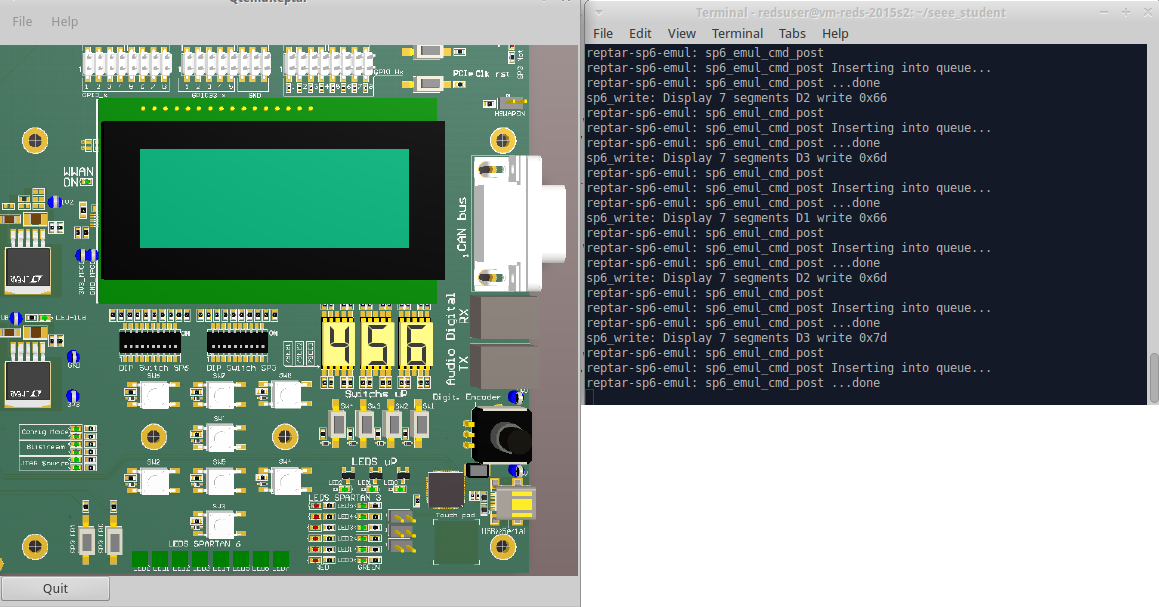
\includegraphics[width=15cm]{img/emulation2.png}
		\caption{Frontend graphique de Qemu avec affichage 7 segments}
		\label{emulation2}
	\end{center}
\end{figure}
\textbf{\color{red}Modifications:\color{black}}\\ Suite à l'examen intermédiaire, nous avons remarqué que nous n'avons pas initialisé correctement la carte Reptar. Nous avons modifié la fonction \textit{sp6\_initfn} du fichier \textit{reptar\_sp6.c} comme ci-dessous. Notre erreur était de passer l'adresse de base du sp6 dans la fonction memory\_region\_init\_io alors que le paramètre demandé était la taille mémoire pour notre périphérique. 
\begin{lstlisting}
//memory_region_init_io(&s->iomem, OBJECT(s), &reptar_sp6_ops, s,
//                  "reptar_sp6", SP6_BASE_ADDRESS);

//Allocate 1MB for reptar
memory_region_init_io(&s->iomem, OBJECT(s), &reptar_sp6_ops, s,
"reptar_sp6", 0x100000);
\end{lstlisting}
Nous avons donc modifié le code pour allouer la bonne taille, soit 1MB, en accord avec la documentation de la plateforme. L'erreur n'a pas eu de conséquence sur les tests, on a juste alloué beaucoup plus de mémoire que nécessaire.\\\\
\textbf{\color{red}Emplacement du code modifié:\color{black}}\textit{/emulationSpartan6\_part6/reptar\_sp6\_modifs.c}
\subsection{Mini-application utilisant les boutons et l'afficheur 7 segments}
\textbf{a) Donnée: }Le dossier miniapp\_u-boot contient un chablon. Complétez-le afin de créer une application qui
utilise les boutons SW2, SW5, SW4 et SW3, ainsi que l’afficheur 7 segments.
\begin{enumerate}
	\item Lors d’un appui sur SW2, SW5 ou SW4, le digit respectivement à gauche, au centre ou au
	milieu est incrémenté de 1, modulo 10. Si un digit atteint 9, il reviendra à 0. 
	\item La valeur initiale de chaque digit, au démarrage de l’application, est 0 (on affichera 000). 
	\item Un appui sur SW3 quitte l’application. 
	\item Vous devrez gérer l’anti-rebond : le digit ne devra être incrémenté que si le bouton est
	pressé puis relâché (comme un appui sur une touche de sonnette par exemple). \\
\end{enumerate}
\textbf{Emplacement du code: }\textit{/miniapp\_test\_emulation/miniapp\_u-boot.c}\\\\
\textbf{Travail réalisé: }L'application a été codée avec une boucle \textit{while} exécutant de manière répétitive les étapes suivantes:
\begin{itemize}
	\item On lit le registre d'état des boutons et on stocke sa valeur dans une première variable. 
	\item On attend un petit moment.
	\item On relit le registre d'état des boutons et on stocke cette nouvelle valeur dans une seconde variable.
	\item Ensuite, on teste les deux variables avec des masques pour savoir si :
	\begin{itemize}
		\item Dans la première variable, le masquage retourne une valeur supérieure à 0 et indique que le bouton testé est enfoncé.
		\item Dans la seconde variable, le masquage retourne une valeur égale à 0 et indique que le bouton a été relâché. 
	\end{itemize}
	Ces tests sont effectués pour les trois boutons d'incrémentation des 7 segments et pour le bouton d'arrêt de l'application. 
	\item Si un des tests passe :
	\begin{itemize}
		\item Si c'est un des boutons d'incrémentation, on appelle la fonction \textit{incr\_7seg} avec en paramètre l'index du 7 segments à incrémenter.
		\item Si c'est le bouton d'arrêt, on quitte la boucle avec un \textit{break}.\\
	\end{itemize}
\end{itemize}
Nous avons remarqué une chose lors de la compilation. Il s'avère que le compilateur prend comme point d'entrée la première instruction du programme, avec le Makefile fourni. Lors des premiers essais, la fonction \textit{incr\_7seg} était implémentée avant le \textit{main}, ce qui en faisait le point d'entrée du programme. Après correction, c'est à dire, définition du prototype de la fonction avant le \textit{main} et implémentation après, tout fonctionne correctement.\\\\
\textbf{b) Donnée: }Testez votre application sur l’émulateur\\\\
\textbf{Travail réalisé: }\\
La figure \ref{emul_miniapp_init} montre l'application qui vient de démarrer. Tous les 7-segments sont initialisés à zero.
\begin{figure}[H]
	\begin{center}
		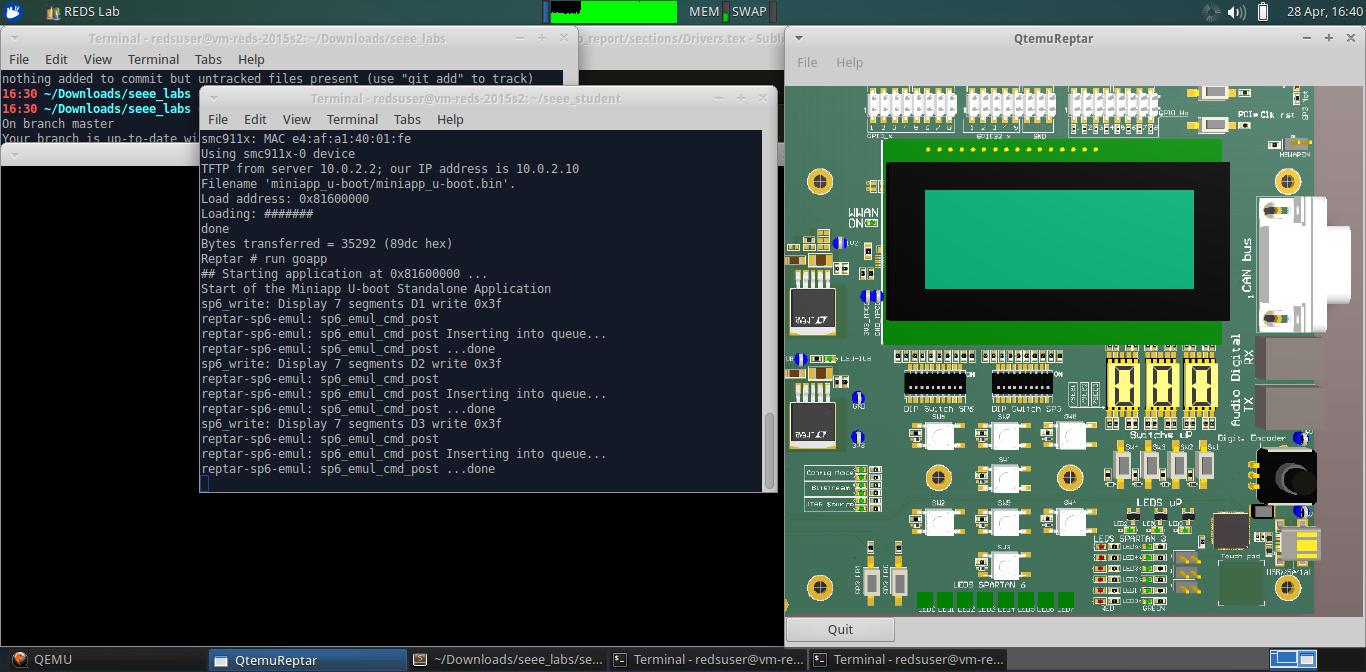
\includegraphics[width=16cm]{img/emul_test_miniapp_init.png}
		\caption{Initialisation des 7-segments durant le lancement de l'application sur le frontend d'émulation}
		\label{emul_miniapp_init}
	\end{center}
\end{figure}
La figure \ref{emul_miniapp_counting} montre l'application avec plusieurs 7-segments incrémentés.
\begin{figure}[H]
	\begin{center}
		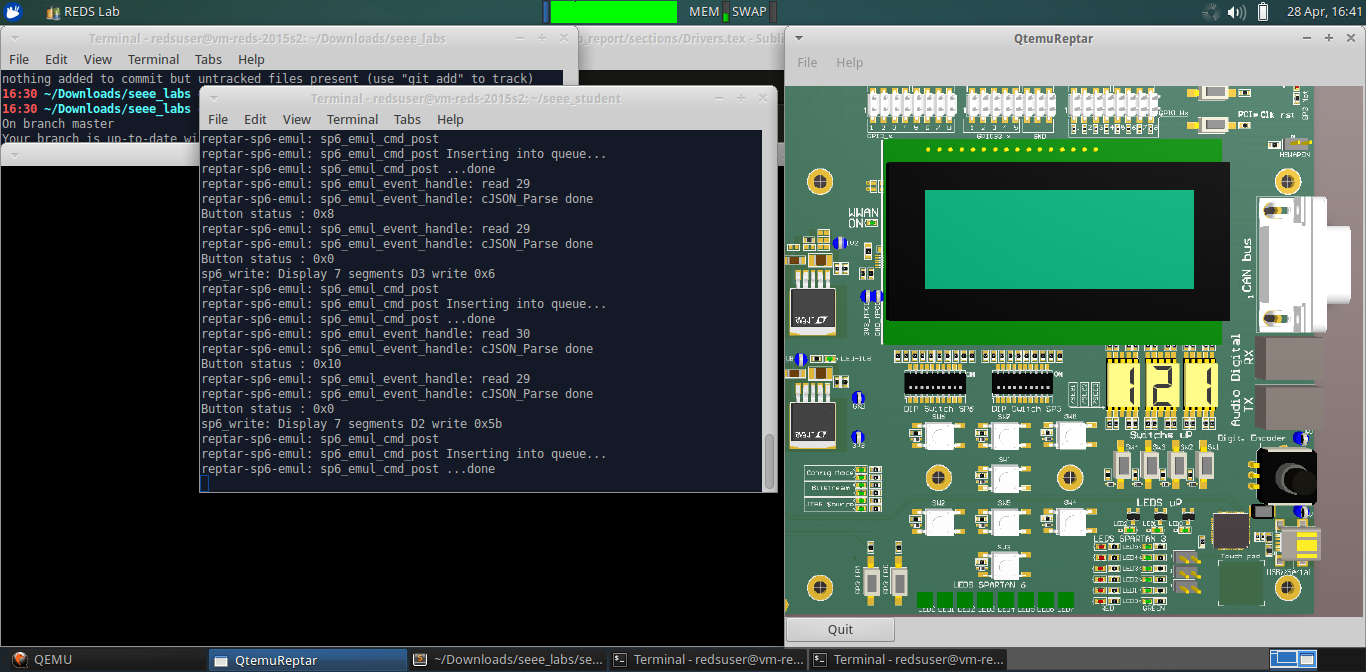
\includegraphics[width=16cm]{img/emul_test_miniapp_counting.png}
		\caption{Incrémentation des 7-segments du frontend d'émulation}
		\label{emul_miniapp_counting}
	\end{center}
\end{figure}
La figure \ref{emul_miniapp_end} montre la fin de l'application. Le bouton tout en bas de la croix a été pressé pour l'arrêter. 
\begin{figure}[H]
	\begin{center}
		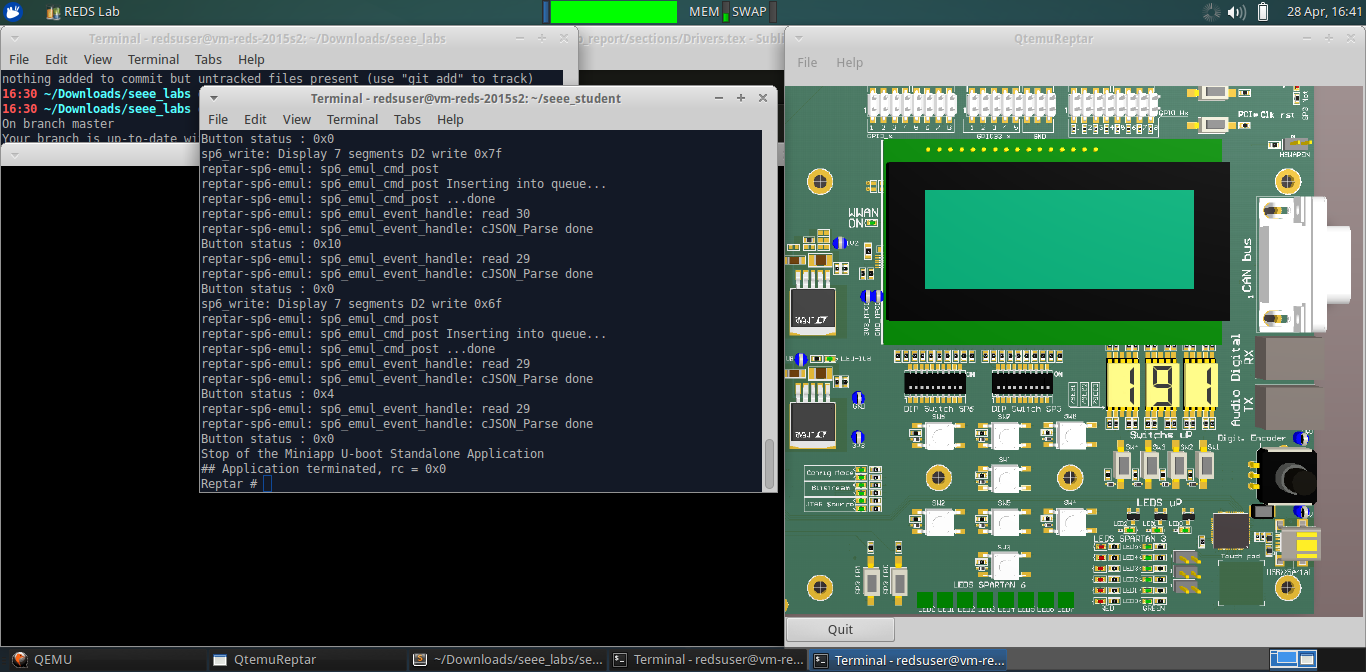
\includegraphics[width=16cm]{img/emul_test_miniapp_end.png}
		\caption{Frontend graphique de Qemu avec affichage 7 segments}
		\label{emul_miniapp_end}
	\end{center}
\end{figure}

\textbf{c) Donnée: }Déployez et testez votre application sur la plate-forme réelle\\\\
\textbf{Travail réalisé: }Une fois l'application compilée, il a fallu copier le \textit{.bin} dans le dossier \textit{tftpboot}. On peut ensuite lancer l'application depuis l'U-boot en accédant la carte Reptar avec \textit{picocom}. La pression sur le switch 3 réussit ici aussi à terminer l'application.
\begin{lstlisting}
$ cd ~/seee_student
$ sudo picocom -b 115200 /dev/ttyUSB0
[sudo] password for redsuser: 
...
Terminal ready

Reptar # tftp 0x81600000 miniapp_u-boot.bin
smc911x: detected LAN9220 controller
smc911x: phy initialized
smc911x: MAC e4:af:a1:40:01:0a
Using smc911x-0 device
TFTP from server 192.168.1.1; our IP address is 192.168.1.10
Filename 'miniapp_u-boot.bin'.
Load address: 0x81600000
Loading: T ###
done
Bytes transferred = 35292 (89dc hex)

Reptar # go 0x81600000
## Starting application at 0x81600000 ...
Start of the Miniapp U-boot Standalone Application
Stop of the Miniapp U-boot Standalone Application
## Application terminated, rc = 0x0
Reptar # 
\end{lstlisting}

Et ici, une photo de l'application en train de tourner sur la plateforme:
\begin{figure}[H]
    \begin{center}
        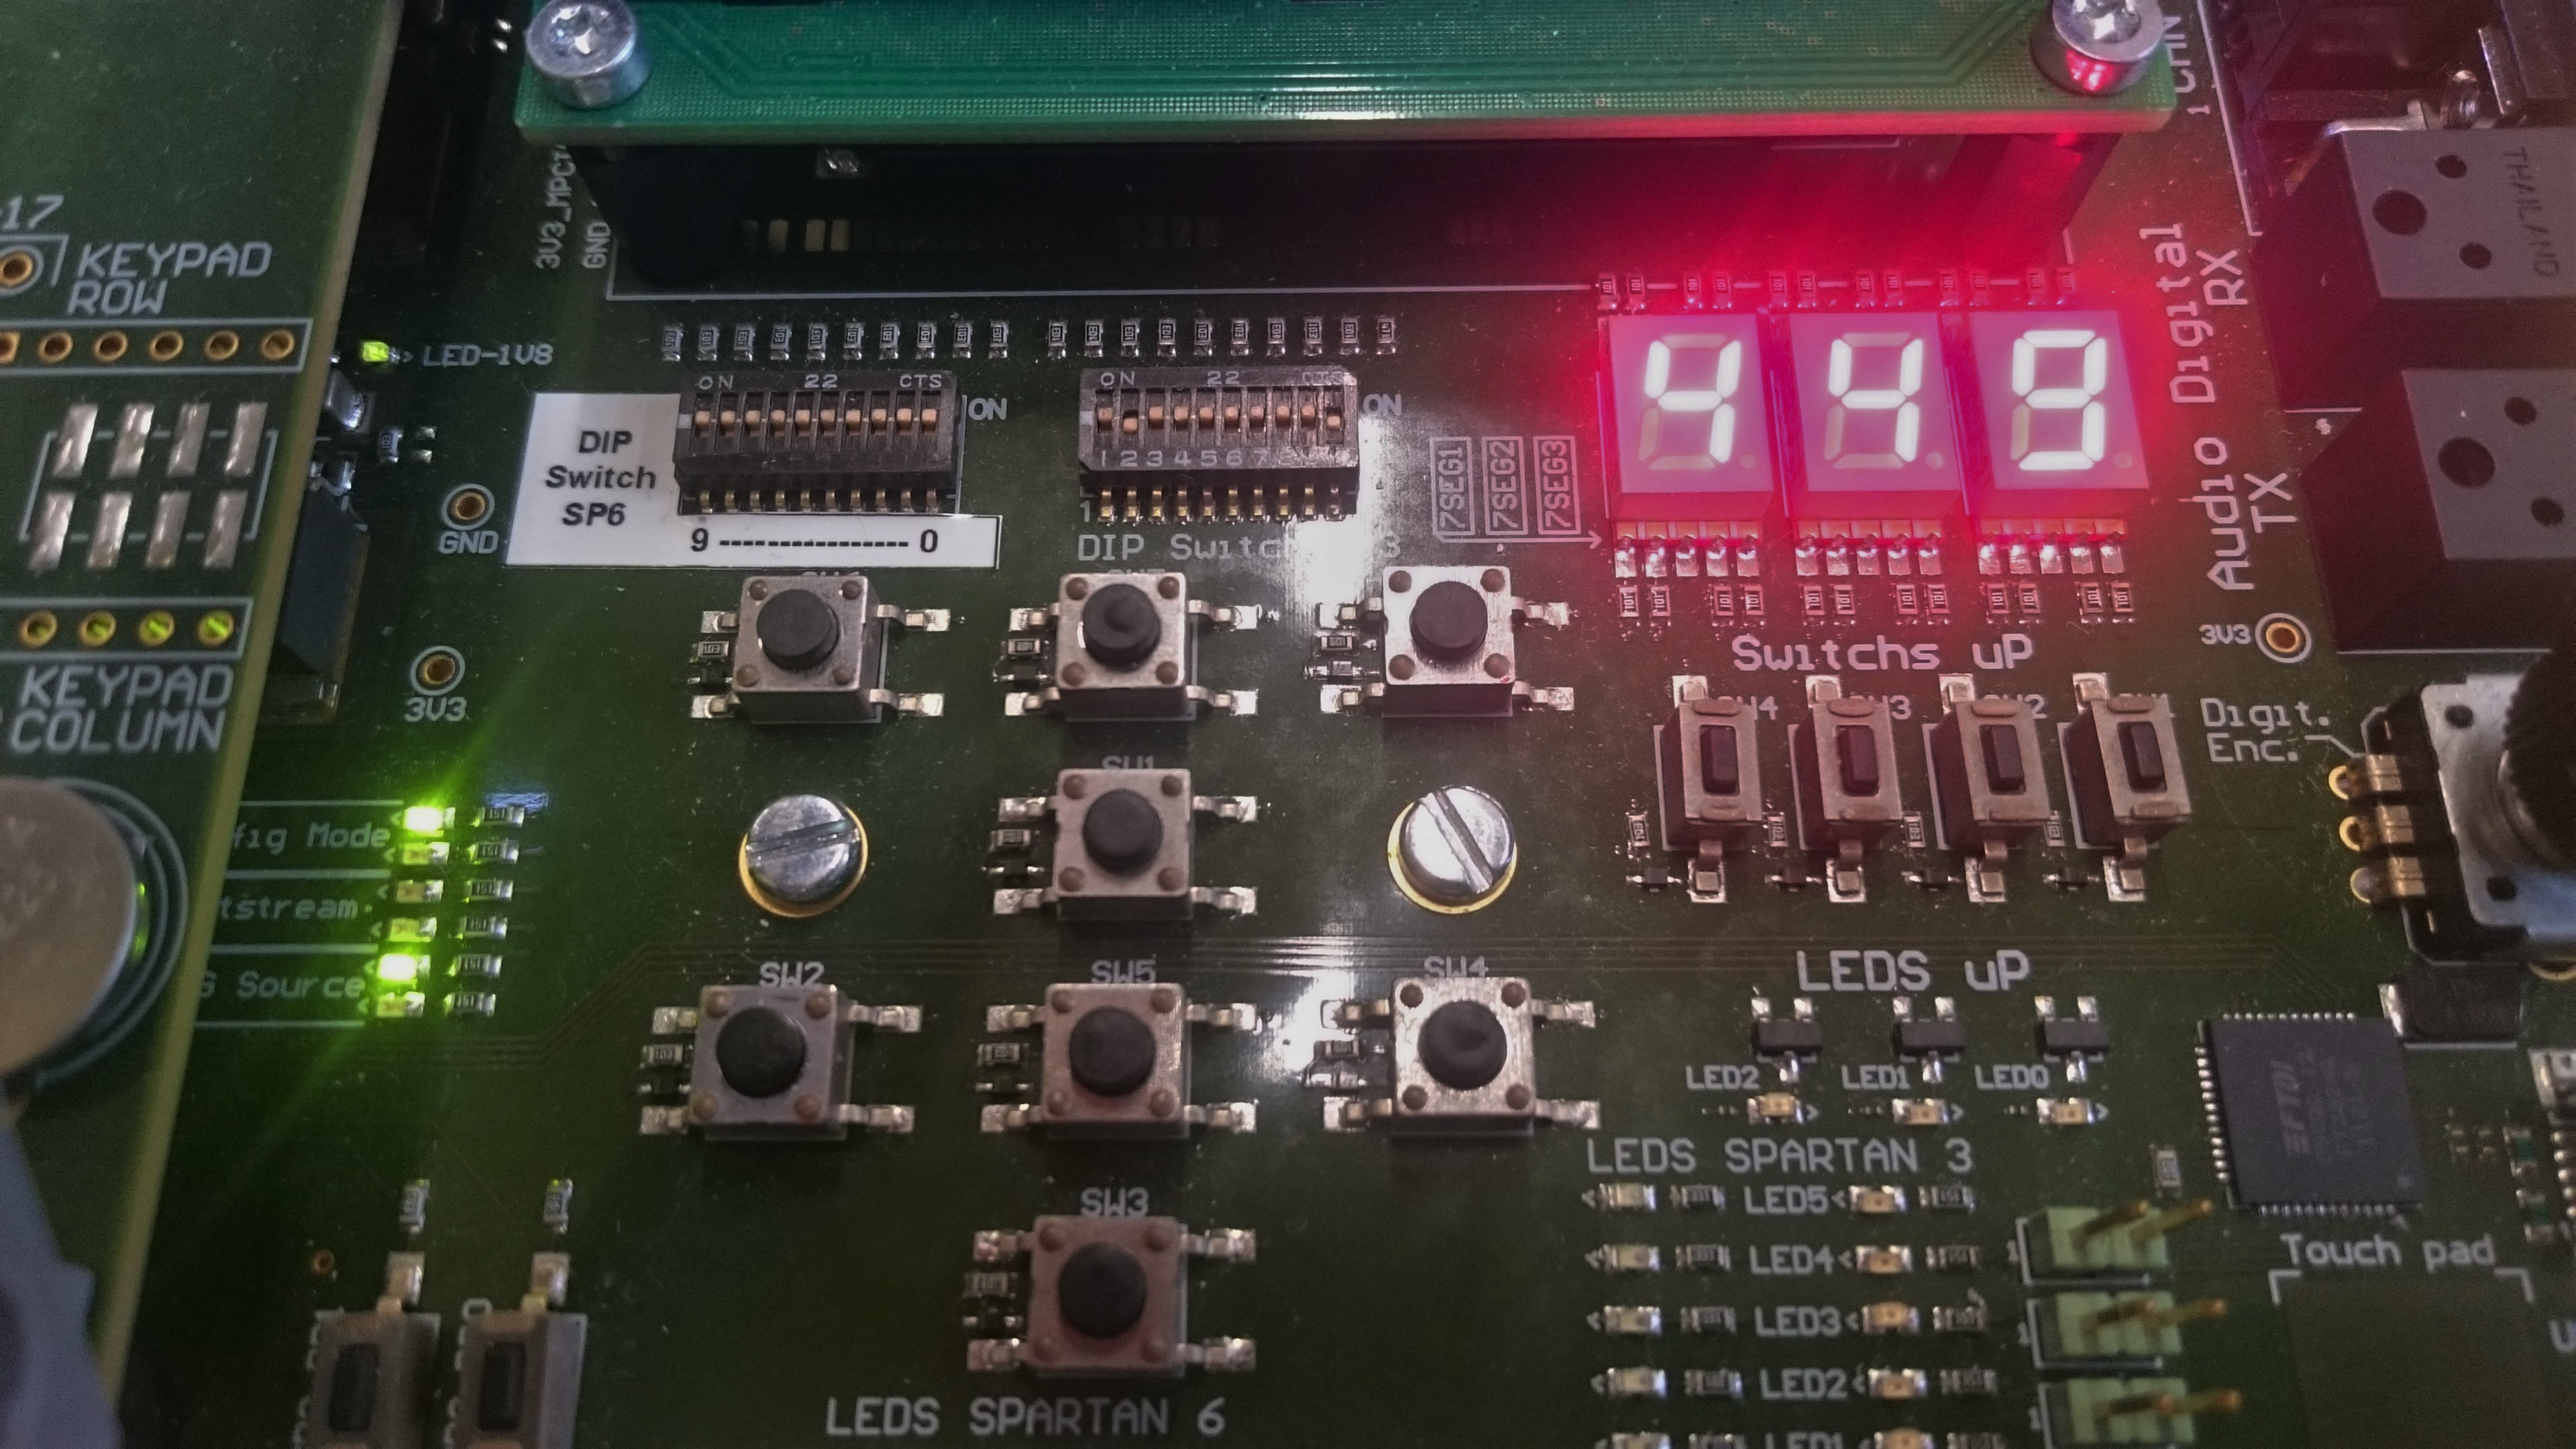
\includegraphics[width=15cm]{img/miniapp_reptar.JPG}
        \caption{Programme miniapp en fonctionnement sur la plateforme physique}
        \label{miniapp_reptar}
    \end{center}
\end{figure}
